\chapter{Evaluation and results} \label{ch:4}

\section{Datasets} \label{s:datasets}

The choice of datasets of protein-ligand complexes used for statistical analysis and P2Rank model training and evaluation was strongly inspired by the datasets described in the P2Rank article \cite{p2rank1}. All structures were re-downloaded directly from PDBe, according to their PDB ID (four-character alphanumeric identifier) and chain ID (one-character identifier) used in the original datasets. It was not possible to take the original datasets as they were, since the structures were not up-to-date and the annotations downloaded from the databases (e.g. feature values) could not be mapped properly.

Furthermore, the re-downloaded datasets were filtered: Obsolete structures were replaced with their current entries, structures that did not have a corresponding UniProt record were removed, as well as  structures with the incorrect segments mapping due to the bug in PDBe (mentioned in Section~\ref{s:mappings}). The pipeline can only work with single-chain structures, and the structures from \textit{holo4k} (see below) and a few structures from \textit{joined} were multi-chain; thus, only one chain was chosen from each such structure.

The resulting datasets were named identically with the original datasets:

\begin{itemize}
  \item \textbf{chen11}
  - a smaller non-redundant dataset that was originally designed for a comparative study of ligand binding sites predictors \cite{benchmark}. It comprises at most one representative chain for every SCOP family \cite{scop} to ensure the minimal sequence similarity and maximal variability in tertiary structure. The original dataset covers 6 structural classes, 148 protein folds, 184 superfamilies and 251 families \cite{benchmark}; after re-downloading and filtering, the numbers are slightly smaller. Although this dataset is rather small, it covers wide range of non-homologous proteins. Therefore, it serves as a good training dataset (P2Rank default model was trained on this dataset as well).
  
  \item \textbf{coach420}
  - a dataset that was originally taken from a benchmark study \cite{cofactor} and used in other studies \cite{coach, p2rank1}. The non-redundant dataset harbors a mix of natural and drug-like ligand molecules.
  
  \item \textbf{joined}
  - a larger dataset created by merging smaller datasets from previous studies. It comprises a set of drug-target complexes extracted from DrugBank, DrugPort and PDB DT198\cite{dt}, a benchmark set for the validation of protein-ligand docking performance \cite{astex}, and a dataset with bound and unbound structures used for evaluation of a ligand binding sites predictor \cite{ligsite}.
  
  \item \textbf{holo4k}
  - a large set of protein-ligand complexes used in a large-scale evaluation of four binding sites predictors \cite{holo4k}.
\end{itemize}


\subsection{Ligands filtering}

The downloaded PDB files contain more ligands per structure, and not all of them are of interest for drug design and other applications. These non-relevant ligands can be ions, peptides, small molecules such as solvents, buffers, detergents and salts that are merely artifacts, and other specific types of ligands.

For each dataset, three variants were created by different filters of the relevant ligands:

\begin{itemize}
\item \textbf{No filter} - Only water molecules were filtered out.
\item \textbf{P2Rank filter} - Relevant ligands were obtained according to the rules used by P2Rank software \cite{p2rank1}. These rules are:
	\begin{itemize}
	\item the ligand has at least 5 atoms
	\item at least one atom of the ligand is in distance 4 {\AA} from any protein atom
	\item the center of the mass of the ligand is not farther than 5.5 {\AA} from the closest protein atom
	\item the name of ligand PDB group is not any of following: HOH, DOD, WAT, NAG, MAN, UNK, GLC, ABA, MPD, GOL, SO4, PO4
	\end{itemize}
\item \textbf{MOAD filter} - Biologically relevant ligands according to the Binding MOAD \cite{moad} database. It contains manually curated crystalography protein-ligand complexes with validated biologically relevant ligands. Only structures obtained by X-ray crystalography with resolution higher than 2.5 {\AA} have entry in Binding MOAD; other structures were removed from the datasets.
\end{itemize}

The structures without any remaining ligands after applying the P2Rank or MOAD filters were removed.

The summary of datasets properties can be seen in Table~\ref{tab:datasets}. The more strict the filter is, the lower the Binding/Non-binding ratio; nevertheless, the information obtained from the relevant binding sites should be more valuable. As we can see, MOAD filter is more strict and filteres out more ligands than P2Rank filter.

\begin{table}[]
\footnotesize
\begin{tabular}{@{}lllllll@{}}
\toprule
Dataset                  & Proteins & Ligands & Lig./Pro. & Binding & Non-bind. & B/N ratio \\ \midrule
chen11                   & 241      & 1039    & 4.3112        & 5670         & 49374            & 0.1148    \\
chen11\_filter\_p2rank   & 223      & 401     & 1.7982        & 4590         & 47073            & 0.0975    \\
chen11\_filter\_MOAD     & 178      & 266     & 1.4944        & 3032         & 39006            & 0.0777    \\
coach420                 & 417      & 841     & 2.0168        & 5988         & 80575            & 0.0743    \\
coach420\_filter\_p2rank & 369      & 427     & 1.1572        & 5247         & 71498            & 0.0734    \\
coach420\_filter\_MOAD   & 258      & 291     & 1.1279        & 3688         & 48485            & 0.0761    \\
joined                   & 527      & 1522    & 2.888         & 8260         & 108337           & 0.0762    \\
joined\_filter\_p2rank   & 446      & 585     & 1.3117        & 6492         & 97158            & 0.0668    \\
joined\_filter\_MOAD     & 348      & 417     & 1.1983        & 4614         & 72363            & 0.0638    \\
holo4k                   & 3973     & 10391   & 2.6154        & 69866        & 790091           & 0.0884    \\
holo4k\_filter\_p2rank   & 3842     & 5049    & 1.3142        & 62483        & 784885           & 0.0796    \\
holo4k\_filter\_MOAD     & 3308     & 4023    & 1.2161        & 50834        & 679918           & 0.0748    \\ \bottomrule
\end{tabular}
\caption[Summary of dataset properties with and without ligands filtering]{Summary of dataset properties with and without ligands filtering. \textit{chen11} dataset has the highest average number of ligands per protein, but when the ligands are filtered, the number is comparable to the other datasets. It indicates that \textit{chen11} has the highest ratio of biologically irrelevant ligands.}
\label{tab:datasets}
\end{table}

\newpage
\section{Statistical analysis}

The statistical analysis of ligand binding sites properties was performed using the analysis pipeline described in Chapter~\ref{ch:3} with default parameters, as described in Attachment~\ref{a:experiments1}. The results were collected for all the datasets, including the versions with filtered ligands.

The results for the datasets with different ligands filters does not seem to differ widely and does not reveal any additional informations. For that reason and for better clarity of the text, following features analysis and plots will be shown only for the datasets with P2Rank ligands filter. The results obtained from the analysis pipeline for all the datasets with and without filters are included in Attachments. TODO odkaz

The P-values computed by the hypothesis tests are shown in Table~\ref{tab:pvaluesAll} and discussed below.

Three artificial features were added for comparison and to check the validity of the tool:
\begin{itemize}
  \item \texttt{lbs} - Ligand binding sites labels (0/1). Should have the best performance of all the features, the P-value should be zero.
  \item \texttt{random\_binary} - Random binary numbers. Should not be significant.
  \item \texttt{random\_cont} - Random continuous feature with values from uniform distribution from 0 to 10. Should not be significant.
\end{itemize}

Some features had to be excluded from the analysis since the data were very sparse and the assumptions of the hypothesis tests would not be met. For example, there were only 15 lipidation sites in the whole \textit{holo4k} dataset containing  857,635 residues. The excluded features are: \texttt{lipidation}, \texttt{glycosylation}, \texttt{non\_standard} and \texttt{compbias}.

The \texttt{conservation} feature was computed only for the three smaller datasets and was omitted for \textit{holo4k}. The computational time would be very high, as it takes 15-30 minutes on average per structure, and the dataset contains almost four thousand proteins. Nevertheless, the comparison on the other three datasets should be sufficient. Furthermore, the computation ended with error for some structures, as there were not enough sequences found by BLAST \cite{blast} (the required number was set to 30).

The problem with feature \texttt{variation} was that the data were missing for many structures (around 3/4) as downloading via REST API resulted in \textit{404 Not Found} error. Data were not available on the UniProt website either. This might be caused by lack of variation data from large-scale studies for some organisms. UniProt helpdesk was contacted to help to explain the issue, but, unfortunately, the question was left without answer. Nevertheless, the feature was analysed on the subset of structures where the data were available.

For some features downloaded from databases, such as \texttt{depth} or \texttt{dynamine}, there were missing data for a few structures as well. These cases were not very frequent and they most likely could not affect the analysis, so they were omitted.


\begin{table}[]
\centering
\begin{tabular}{@{}lllll@{}}
\toprule
{\color[HTML]{000000} }       & {\color[HTML]{000000} \textbf{chen11}} & {\color[HTML]{000000} \textbf{coach420}} & {\color[HTML]{000000} \textbf{joined}} & {\color[HTML]{000000} \textbf{holo4k}} \\ \midrule
\textbf{lbs (test)}                  & 0                                      & 0                                        & 0                                      & 0                                      \\
\textbf{pdbekb\_conservation} & 0                                      & 0                                        & 0                                      & 0                                      \\
\textbf{conservation}         & 0                                      & 0                                        & 0                                      & X                                      \\
\textbf{HSE\_up}              & 0                                      & 0                                        & 0                                      & 0                                      \\
\textbf{exposure\_CN}         & 1.43E-278                              & 0                                        & 0                                      & 0                                      \\
\textbf{depth}                & 1.26E-241                              & 1.38E-251                                & 0                                      & 0                                      \\
\textbf{HSE\_down}            & 8.20E-158                              & 1.99E-244                                & 0                                      & 0                                      \\
\textbf{bfactor}              & 3.79E-197                              & 1.12E-143                                & 0                                      & 0                                      \\
\textbf{mol\_weight}          & 4.70E-143                              & 7.15E-136                                & 1.16E-245                              & 0                                      \\
\textbf{aa}                   & 3.96E-143                              & 1.80E-137                                & 7.54E-245                              & 0                                      \\
\textbf{hydropathy}           & 2.83E-139                              & 4.26E-137                                & 1.40E-244                              & 0                                      \\
\textbf{aromaticity}          & 1.17E-78                               & 1.56E-57                                 & 3.05E-111                              & 0                                      \\
\textbf{H\_bond\_atoms}       & 6.57E-53                               & 2.85E-49                                 & 8.00E-109                              & 0                                      \\
\textbf{sec\_str}             & 1.44E-17                               & 1.34E-52                                 & 4.66E-44                               & 0                                      \\
\textbf{polarity}             & 5.99E-10                               & 6.97E-25                                 & 5.31E-37                               & 0                                      \\
\textbf{charged}              & 8.28E-11                               & 2.45E-25                                 & 9.96E-29                               & 0                                      \\
\textbf{strand}               & 4.24E-18                               & 9.51E-35                                 & 1.74E-44                               & 4.40E-279                              \\
\textbf{helix}                & 1.45E-07                               & 1.01E-35                                 & 3.23E-16                               & 1.21E-268                              \\
\textbf{disulfid}             & \cellcolor[HTML]{F54D4D}0.353          & 4.29E-07                                 & \cellcolor[HTML]{F54D4D}0.1728         & 2.16E-94                               \\
\textbf{mod\_res}             & \cellcolor[HTML]{F54D4D}0.362          & 0.004458                                 & 0.000132                               & 5.95E-55                               \\
\textbf{mobiDB}               & 1.22E-06                               & 0.0004838                                & 7.91E-13                               & 9.73E-54                               \\
\textbf{cis\_peptide}         & \cellcolor[HTML]{F54D4D}0.1914         & 9.85E-05                                 & 2.63E-05                               & 1.06E-48                               \\
\textbf{natural\_variant}     & \cellcolor[HTML]{F54D4D}0.7951         & 0.000333                                 & 1.19E-05                               & 7.46E-45                               \\
\textbf{PTM}                  & \cellcolor[HTML]{F54D4D}0.8162         & 0.04154                                  & 0.007383                               & 1.83E-38                               \\
\textbf{phi\_angle}           & 1.91E-05                               & 2.85E-05                                 & 6.08E-08                               & 6.68E-37                               \\
\textbf{psi\_angle}           & 0.02216                                & 1.79E-15                                 & 0.002092                               & 2.58E-20                               \\
\textbf{efoldmine}            & 0.0001874                              & 0.001525                                 & 7.54E-23                               & 2.51E-14                               \\
\textbf{dynamine}             & 0.007162                               & 0.01094                                  & 1.26E-07                               & 0.0003708                              \\
\textbf{variation}            & \cellcolor[HTML]{F54D4D}0.1864         & \cellcolor[HTML]{F54D4D}0.2724           & 0.01176                                & 0.004204                               \\
\textbf{turn}                 & \cellcolor[HTML]{F54D4D}0.6574         & 0.00167                                  & \cellcolor[HTML]{F54D4D}0.5149         & 0.03571                                \\
\textbf{random\_cont (test)}         & \cellcolor[HTML]{F54D4D}0.8255         & \cellcolor[HTML]{F54D4D}0.9688           & \cellcolor[HTML]{F54D4D}0.9748         & \cellcolor[HTML]{F54D4D}0.6919         \\
\textbf{random\_binary (test)}       & 0.04112                                & \cellcolor[HTML]{F54D4D}0.1669           & \cellcolor[HTML]{F54D4D}0.1722         & \cellcolor[HTML]{F54D4D}0.7793         \\ \bottomrule
\end{tabular}
\caption[P-values returned by hypothesis tests for individual features]{P-values returned by hypothesis tests for individual features for all four datasets (with P2Rank ligands filtering). Features are sorted according to the values for \textit{holo4k}. Values highlighted with red colour are higher that the significance level $\alpha = 0.05$.\\\hspace{\textwidth}
*\texttt{variation} is computed only on the small subsets of proteins for which the data were available in databases.}
\label{tab:pvaluesAll}
\end{table}

As we can see from the results in Table~\ref{tab:pvaluesAll}, most features appear to be statistically significant, having the P-value below the significance level $\alpha=0.05$.
The results for the test features \texttt{lbs}, \texttt{random\_binary} and \texttt{random\_cont} seem to be valid. Nevertheless, when looking at the histograms and plots, some results are not as expected. Let's take a look at the histogram depicted in Figure~\ref{fig:dynamine}: the distribution of \texttt{dynamine} values does not seem significantly different in binding and non-binding sites. Note that for better comparison of binding and non-binding sites (since their ratio is very unbalanced), the density is computed with respect to the number of binding or non-binding sites; the value in the histogram bin can be understood as conditional probability of getting that value when having a binding/non-binding residue.

\begin{figure}[]
\centering
\includegraphics[width=120mm]{../img/dynamine_hist.png}
\caption[Histogram for feature \texttt{dynamine}]{Histogram for feature \texttt{dynamine} computed on \textit{holo4k} dataset. Density on the y-axis is computed with respect to the number of binding or non-binding sites. Difference in means: 0.0012.}
\label{fig:dynamine}
\end{figure}

One conspicuous thing about the Table~\ref{tab:pvaluesAll} is that, in general, the P-values are getting smaller as the dataset size grows (the datasets in the table are sorted from the smallest on the left to the largest on the right). This is referred to as the \textit{P-value problem}. For very large samples, the statistical power of hypothesis tests is higher, and causes P-value going to zero. When dealing with large samples, even the miniscule effects can become statistically significant. The test can detect subtler and more complex effects, which can be advantageous in some cases, but also misleading. It all depends on the purpose of the statistical testing. The question we should ask is not whether the results are statistically significant (which there almost always is for large samples), but whether they are interesting for our research \cite{pvalueproblem}.

Let's see the P-value problem demonstrated on our data. Figure~\ref{fig:pvalueDeflation} shows different speeds of P-value deflation for chosen features. The computation of the plots was inspired by `Monte Carlo CPS Charts' described by Lin \textit{et al.} \cite{pvalueproblem}. For feature \texttt{exposure\_CN}, sample size of 50 is sufficient to get P-values below significance level 0.05. We can clearly see from the histogram that the values in binding and non-binding sites differ, so this is an expected result. On the contrary, the values of feature \texttt{dynamine} does not seem to differ significantly for binding and non-binding sites, and yet, if the sample size is large enough, we get statistically significant result.

\begin{figure}[]
\centering
\begin{subfigure}[b]{\textwidth}
  \centering
  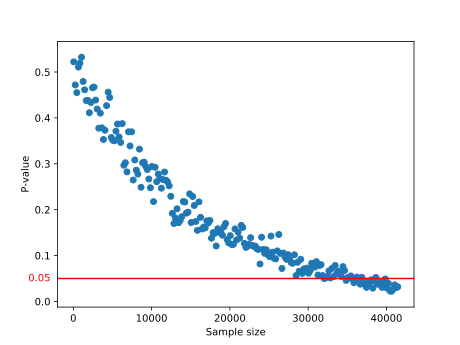
\includegraphics[width=0.475\linewidth]{../img/pValue_deflation_dynamine.pdf}%
  \includegraphics[width=0.475\linewidth]{../img/dynamine_hist.png}
  \caption{\texttt{dynamine}}
\end{subfigure}
\vskip\baselineskip
\begin{subfigure}[b]{\textwidth}
  \centering
  \includegraphics[width=0.475\linewidth]{../img/pValue_deflation_phi_angle.pdf}%
  \includegraphics[width=0.475\linewidth]{../img/phi_angle_hist.png}
  \caption{\texttt{phi\_angle}}
\end{subfigure}
\vskip\baselineskip
\begin{subfigure}[b]{\textwidth}
  \centering
  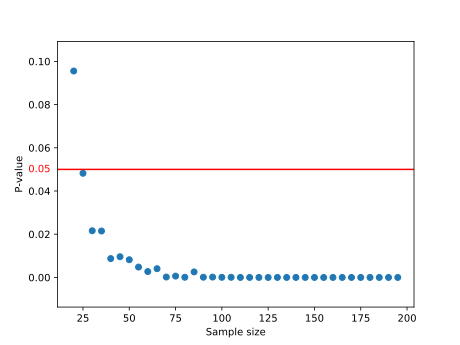
\includegraphics[width=0.475\linewidth]{../img/pValue_deflation_exposure_CN.pdf}%
  \includegraphics[width=0.475\linewidth]{../img/exposure_CN_hist.png}
  \caption{\texttt{exposure\_CN}}
\end{subfigure}
\caption[P-value deflation]{Different speed of P-value deflation demonstrated on three features. The P-value decreases with increasing sample size. The results were obtained from 100 iterations of random sampling with given sample size, taking the same number of binding and non-binding residues. Mean P-values and standard deviations are displayed (the error bars are cut so they are not negative). Computed on dataset \textit{holo4k} with P2Rank ligands filter. The red line represents significance level $\alpha=0.05$. }
\label{fig:pvalueDeflation}
\end{figure}

To complement the hypothesis tests and to provide an objective measure of importance of the results, we report two effect size measures, as described in Section~\ref{s:effectsize}: Cohen's \textit{d} for continuous features and Cohen's \textit{w} for the rest. The results can be found in Table~\ref{tab:cohensd} and Table~\ref{tab:cohensw}. Looking at the effect sizes, it seems that many low P-values reported in Table~\ref{tab:pvaluesAll} are most likely mere artifacts of the large sample sizes. Only a few features seem to have any practical significance. The individual features will be discussed below.

% Please add the following required packages to your document preamble:
% \usepackage{booktabs}
\begin{table}[]\centering
\begin{tabular}{@{}lllll@{}}
\toprule
                      & \textbf{chen11} & \textbf{coach420} & \textbf{joined} & \textbf{holo4k} \\ \midrule
\textbf{conservation} & 0.7726          & 0.9009            & 0.8083          & X               \\
\textbf{exposure\_CN} & 0.6161          & 0.7419            & 0.8181          & 0.839           \\
\textbf{depth}        & 0.6666          & 0.6308            & 0.8569          & 0.8255          \\
\textbf{HSE\_up}      & 0.5772          & 0.6512            & 0.7513          & 0.7373          \\
\textbf{HSE\_down}    & 0.4424          & 0.5236            & 0.5874          & 0.5895          \\
\textbf{bfactor}      & 0.3959          & 0.3207            & 0.3872          & 0.4382          \\
\textbf{phi\_angle}   & 0.06842         & 0.06729           & 0.07535         & 0.0592          \\
\textbf{mobiDB}       & 0.06575         & 0.04492           & 0.07718         & 0.05498         \\
\textbf{psi\_angle}   & 0.03685         & 0.1209            & 0.04151         & 0.04111         \\
\textbf{efoldmine}    & 0.06121         & 0.0491            & 0.1455          & 0.03436         \\
\textbf{dynamine}     & 0.04341         & 0.04098           & 0.07485         & 0.01685         \\
\textbf{random\_cont (test)} & 0.003419        & 0.00056           & 0.0004042       & 0.001647        \\ \bottomrule
\end{tabular}
\caption[Values of Cohen's \textit{d}]{Values of Cohen's \textit{d} for continuous features. Features are sorted according to the values for \textit{holo4k}.}
\label{tab:cohensd}
\end{table}

% Please add the following required packages to your document preamble:
% \usepackage{booktabs}
\begin{table}[] \centering
\begin{tabular}{@{}lllll@{}}
\toprule
\textbf{}                     & \textbf{chen11} & \textbf{coach420} & \textbf{joined} & \textbf{holo4k} \\ \midrule
\textbf{lbs (test)}                  & 0.9999          & 0.9999            & 0.9999          & 1               \\
\textbf{pdbekb\_conservation} & 0.341           & 0.3266            & 0.3149          & 0.349           \\
\textbf{aa}                   & 0.1191          & 0.09592           & 0.108           & 0.1127          \\
\textbf{mol\_weight}          & 0.1188          & 0.09515           & 0.108           & 0.1124          \\
\textbf{hydropathy}           & 0.1167          & 0.09502           & 0.1074          & 0.1113          \\
\textbf{H\_bond\_atoms}       & 0.07016         & 0.05561           & 0.07041         & 0.07102         \\
\textbf{aromaticity}          & 0.08261         & 0.05771           & 0.06961         & 0.06377         \\
\textbf{sec\_str}             & 0.03977         & 0.05644           & 0.04458         & 0.04623         \\
\textbf{polarity}             & 0.02867         & 0.03807           & 0.04015         & 0.04574         \\
\textbf{charged}              & 0.02858         & 0.03755           & 0.03454         & 0.04437         \\
\textbf{strand}               & 0.03819         & 0.04444           & 0.04363         & 0.03883         \\
\textbf{helix}                & 0.02316         & 0.04509           & 0.02546         & 0.03809         \\
\textbf{disulfid}             & 0.00409         & 0.01827           & 0.004251        & 0.02242         \\
\textbf{mod\_res}             & 0.004014        & 0.01028           & 0.01192         & 0.01698         \\
\textbf{cis\_peptide}         & 0.005721        & 0.01404           & 0.01304         & 0.01592         \\
\textbf{natural\_variant}     & 0.001144        & 0.01297           & 0.01366         & 0.01528         \\
\textbf{PTM}                  & 0.001024        & 0.007366          & 0.008354        & 0.01411         \\
\textbf{variation}            & 0.01132         & 0.008884          & 0.01283         & 0.005528        \\
\textbf{turn}                 & 0.001953        & 0.01136           & 0.00203         & 0.002284        \\
\textbf{random\_binary (test)}       & 0.008985        & 0.00499           & 0.00424         & 0.0003044       \\ \bottomrule
\end{tabular}
\caption[Values of Cohen's \textit{w}]{Values of Cohen's \textit{w} for binary, ordinal and categorical features. Features are sorted according to the values for \textit{holo4k}.}
\label{tab:cohensw}
\end{table}

Another noticeable thing about Table~\ref{tab:pvaluesAll} is that the results for some features vary across datasets. Let's take a look at features \texttt{disulfid} and \texttt{turn}, for example. The P-value is very high for datasets \textit{chen11} and \textit{joined}; contrarily, it is low for \textit{coach420} and \textit{holo4k}. In this case it is not true that the P-value would decrease with the increasing sample size. This leads to a question of how the datasets are composed, and whether they are representative samples from the whole population of proteins. Taken into consideration the way how the datasets were assembled, it is likely that some bias was introduced. The question is whether taking the whole PDB database would help to solve this issue. There probably would be the problem with redundancy of data, as close homologs and overlapping PDB entries would be included. Furthermore, the database itself is most likely a biased sample of the real world of proteins, as the tertiary structure is yet to be discovered for many of them. And most importantly, this approach would be computationally very demanding.


\section{Statistical analysis - random sampling}

To make use of our large datasets, one different approach was implemented. Dataset \textit{mix} was created by merging all four datasets together, removing a few duplicates. The dataset contains a total number of 5047 structures. Random sampling without replacement was applied on this dataset, in each iteration taking a sample of 500 binding and 500 non-binding sites without replacement. 1000 iterations were executed and mean effect sizes were reported. The prodecure is described in Attachment~\ref{a:experiments2}. The resulting effect sizes are shown in Table~\ref{tab:cohensd500} and Table~\ref{tab:cohensw500}.

This approach has the advantage of removing possible dependencies of nearby residues. For many features, the values of individual residues are not independent of each other. For instance, a helix or a beta sheet always covers several consecutive residues. The features obtained from the structure, such as different measures of burriedness (e.g. \texttt{exposure\_CN}, \texttt{depth}) can have similar values for spacially near residues. And the features computed from the FASTA sequence, such as \texttt{dynamine} or \texttt{mobiDB}, most likely have some dependencies as well, from the principle of their computation. When taking a small sample of 500 residues, the chance of these dependencies affecting the analysis is minimal.

The sample size of 500 was chosen for two reasons: firstly, validity of the Central Limit Theorem needs to be assured, as described in Section~\ref{s:welchs}. Lumley \textit{et al.} \cite{lumley} demonstrated that 500 is a sufficiently large sample even for extremely non-normal data. And secondly, the minimum sample size assuring the Central Limit Theorem validity should be chosen, to avoid the P-value problem. Smaller sample size would probably be sufficient for the Central Limit Theorem, as 500 is a very safe estimation. Nevertheless, the sample size could not be much smaller anyhow, since the data for some categorial features would be very sparse. Even with the sample size of 500, features \texttt{PTM}, \texttt{mod\_res}, \texttt{natural\_variant}, \texttt{disulfid} and \texttt{cis\_peptide} needed to be excluded from the analysis, as there was not sufficient number of positives in this smaller sample.

\begin{table}[]
\centering
\begin{tabular}{@{}llc@{}}
\toprule
                      & \textbf{mean} & \textbf{standard deviation} \\ \midrule
\textbf{conservation} & 0.8812        & 0.06919           \\
\textbf{exposure\_CN} & 0.7829        & 0.06753           \\
\textbf{HSE\_up}      & 0.7511        & 0.06866           \\
\textbf{depth}        & 0.6927        & 0.06815           \\
\textbf{HSE\_down}    & 0.5649        & 0.06453           \\
\textbf{bfactor}      & 0.4744        & 0.06165           \\
\textbf{phi\_angle}   & 0.07136       & 0.05012           \\
\textbf{mobiDB}       & 0.07066       & 0.04874           \\
\textbf{psi\_angle}   & 0.06029       & 0.045             \\
\textbf{efoldmine}    & 0.05961       & 0.04477           \\
\textbf{dynamine}     & 0.05236       & 0.04086           \\
\textbf{random\_cont (test)} & 0.04968       & 0.03807           \\ \bottomrule
\end{tabular}
\caption[Mean effect sizes (cohen's \textit{d})]{Mean effect sizes (cohen's \textit{d}) computed from 1000 iterations of random sampling with sample size 500. Computed on dataset \textit{mix} (all 4 datasets merged together) with P2Rank ligands filter. Features are sorted according to the effect size.}
\label{tab:cohensd500}
\end{table}

\begin{table}[!h]
\centering
\begin{tabular}{@{}llc@{}}
\toprule
                              & \textbf{mean} & \textbf{standard deviation} \\ \midrule
\textbf{lbs (test)}                  & 0.998         & 2.22E-16                    \\
\textbf{pdbekb\_conservation} & 0.4742        & 0.02518                     \\
\textbf{aa}                   & 0.2443        & 0.02677                     \\
\textbf{mol\_weight}          & 0.2414        & 0.0259                      \\
\textbf{hydropathy}           & 0.2336        & 0.02724                     \\
\textbf{H\_bond\_atoms}       & 0.1411        & 0.02893                     \\
\textbf{aromaticity}          & 0.1067        & 0.03028                     \\
\textbf{sec\_str}             & 0.09798       & 0.02917                     \\
\textbf{polarity}             & 0.09157       & 0.0296                      \\
\textbf{charged}              & 0.08189       & 0.032                       \\
\textbf{strand}               & 0.07289       & 0.03048                     \\
\textbf{helix}                & 0.07052       & 0.02998                     \\
\textbf{random\_binary (test)}       & 0.02375       & 0.01976                     \\
\textbf{variation}            & 0.02298       & 0.01929                     \\
\textbf{turn}                 & 0.02023       & 0.01797                     \\ \bottomrule
\end{tabular}
\caption[Mean effect sizes (cohen's \textit{w})]{Mean effect sizes (cohen's \textit{w}) computed from 1000 iterations of random sampling with sample size 500. Computed on dataset \textit{mix} (all 4 datasets merged together) with P2Rank ligands filter. Features are sorted according to the effect size.
\hspace{\textwidth}
*\texttt{variation} is computed only on the subsets of proteins for which the data were available in databases.}
\label{tab:cohensw500}
\end{table}

\newpage
\section{Discussion}
Let's discuss the results from the two previous sections in more detail.

The results for both conservation features \texttt{conservation} and \texttt{pdbekb\_conservation} turned out as expected. Sequence conservation has been used previously in many approaches for protein-ligand binding sites prediction and its importance for the prediction has been repeatedly demonstrated \cite{ligsite, cons, casp, prankweb}. The higher values of conservation for binding residues are clearly visible from the Figure~\ref{fig:conservation}. The effect sizes are the highest from all the examined features and it seems that the sequence conservation might be even more correlated with binding sites positions than the locations of cavities on the protein surface.

\begin{figure}[!h]
\centering
\begin{subfigure}{.5\textwidth}
  \centering
  \includegraphics[width=1\linewidth]{../img/conservation_hist.png}
  \caption{\texttt{conservation}}
\end{subfigure}%
\begin{subfigure}{.5\textwidth}
  \centering
  \includegraphics[width=1\linewidth]{../img/pdbekb_conservation_frequencies.png}
  \caption{\texttt{pdbekb\_conservation}}
\end{subfigure}
\caption[Conservation features]{Higher values of conservation for binding residues demonstrated on two features: (a) continuous feature computed by the P2Rank conservation pipeline, and (b) ordinal feature downloaded from PDBe-KB database.}
\label{fig:conservation}
\end{figure}

Features \texttt{HSE\_up}, \texttt{HSE\_down}, \texttt{exposure\_CN} and \texttt{depth} are closely related to the `buriedness' of the residue. Similarly as conservation, this feature was expected to be important for ligand binding sites recognition. Many binding sites are shaped as cavities, or concave pockets, on the surface of the 3D structure. The geometrical methods, such as LIGSITE \cite{ligsite} or PocketPicker \cite{pocketpicker}, as well as other approaches (including P2Rank), make use of this property (as explained in Section~\ref{s:existingmethods}. The histograms for these continuous features are depicted in Figure~\ref{fig:buriedness}. The effect sizes for all four features indicate quite large effect.


\begin{figure}[]
\centering
\begin{subfigure}{.5\textwidth}
  \centering
  \includegraphics[width=1\linewidth]{../img/exposure_CN_hist.png}
  \caption{\texttt{exposure\_CN}}
\end{subfigure}%
\begin{subfigure}{.5\textwidth}
  \centering
  \includegraphics[width=1\linewidth]{../img/depth_hist.png}
  \caption{\texttt{depth}}
\end{subfigure}
\begin{subfigure}{.5\textwidth}
  \centering
  \includegraphics[width=1\linewidth]{../img/HSE_up_hist.png}
  \caption{\texttt{HSE\_up}}
\end{subfigure}%
\begin{subfigure}{.5\textwidth}
  \centering
  \includegraphics[width=1\linewidth]{../img/HSE_down_hist.png}
  \caption{\texttt{HSE\_down}}
\end{subfigure}
\caption[The features related to the `buriedness']{The features related to the residue `buriedness' have higher values in binding sites.}
\label{fig:buriedness}
\end{figure}

The analysis reveals that binding sites have slightly lower B factor values on average (see Figure~\ref{fig:bfactor}). This could indicate that binding sites are more well-ordered in general, whereas non-binding sites might have higher flexibility.

\begin{figure}[]
\centering
\includegraphics[width=0.7\linewidth]{../img/bfactor_hist.png}
\caption[Feature \texttt{bfactor}]{\texttt{bfactor}: Binding sites seem to have lower B factor values, which could indicate bigger rigidity of binding sites.}
\label{fig:bfactor}
\end{figure}

Binding and non-binding sites seem to have different residue composition. Let's take a look at Figure~\ref{fig:aa}. Cys, Trp, Phe, Tyr, Gly, His, Met and Ile all have high binding/non-binding ratios, and thus, are more likely to occur in binding sites. On the other hand, Pro, Glu, Gln, Lys and Asp disfavour binding sites. Arg, Val, Ser and Leu are very frequent in binding sites; however, they have the ratios similar to the total binding/non-binding ratio, as they are very frequent on the whole protein surface, not only in binding sites. This result is in accordance with a large-scale study that explored the composition of protein-ligand binding sites \cite{lbscomposition}. This is an interesting result; nevertheless, the effect size is smaller than for the previously discussed features and it is not clear whether the tendency of some amino acids to appear in the binding sites with higher frequency could be used for the prediction.

\begin{figure}[]
\centering
\begin{subfigure}{\textwidth}
  \centering
  \includegraphics[width=0.7\linewidth]{../img/aa_frequencies.png}
  \caption{Frequencies of individual amino acids in binding and non-binding sites.}
\end{subfigure}
\begin{subfigure}{\textwidth}
  \centering
  \includegraphics[width=0.7\linewidth]{../img/aa_ratios.png}
  \caption{Comparison of binding/non-binding ratios, computed as occurrences of the AA in binding sites divided by its occurrences in non-binding sites. The red line marks the total binding/non-binding ratio (total number of binding sites divided by total number of non-binding sites). High ratio means that the AA favours binding sites, and on the contrary, the low ratio indicates the tendency to occur in non-binding sites.}
\end{subfigure}
\caption[Feature \texttt{aa}]{Feature \texttt{aa}.}
\label{fig:aa}
\end{figure}

The molecular weight and hydropathy seem to have similar effect as the amino acid composition. This result is most probably caused by the fact that the values of the molecular weight and the hydropathy index correlate with the amino acid labels almost completely. To explain it more clearly, \texttt{mol\_weight} is an ordinal feature with 19 categories, where one category means one value of molecular weight for one amino acid (only leucine and isoleucine have the same molecular weight and thus fall into the same category). It means that computing this feature is almost equivalent to computing feature \texttt{aa}, only with different labels for categories and two amino acids merged into one category. The feature \texttt{hydropathy} is similar, only with 17 categories. The rest of amino acid-based features does not have this characteristic, as they are either binary (\texttt{charged}, \texttt{aromaticity}) or with small number of categories (\texttt{polarity}, \texttt{H\_bond\_atoms}).

The rest of the features does not seem to be very important for binding sites differetiation, as the effects are very small or negligible. \texttt{aromaticity} and \texttt{H\_bond\_atoms} features look the most promising of the rest and could be given a try. None of properties such as torsion angles, secondary structures, disorder regions, polarity and charge of a residue, early folding regions or regions with increased backbone dynamics appear to have significantly different value within the binding sites. This means that unfortunately, the analysis has not revealed any novel features that would help to increase the protein-ligand binding sites prediction.

\newpage

\section{P2Rank models}

The features examined in the previous sections were used to train new P2Rank models and to find out their practical significance. All models were trained with the same parameters as the default P2Rank model (100 trees, each grown with no depth limit using 6 features). The models were trained on \textit{chen11} dataset and evaluated on \textit{coach420} dataset. The training was done with parameter \texttt{loop=10} which means that the model was trained 10 times, every time with different random seed, and the performances of the 10 resulting models were averaged at the end. This is important for reducing the influence of the random behaviour of the classifier. The procedure is described in Attachment~\ref{a:experiments3}.

The features obtained by the analysis pipeline are called `csv features' in the following section, in accordance with the terminology used by P2Rank for user-defined features in csv files.

A couple of features were left out from the following experiments. The feature \texttt{variation} had missing values for around 3/4 structures, as mentioned in the previous section, and the comparison with the rest of the features would not make much sense. Categorical feature \texttt{aa} was replaced by 20 binary features representing individual amino acids (\texttt{aa\_HIS}, \texttt{aa\_SER} etc.). Similarly, categorical feature \texttt{sec\_str} was left out and represented by features \texttt{helix}, \texttt{strand} and \texttt{turn}.

The performance of the baseline model (trained with all default P2Rank features and no csv feature) was compared with the model trained with all csv features (test features \texttt{lbs}, \texttt{random\_binary} and \texttt{random\_cont} were left out of course), and the model trained with both P2Rank features and csv features. The results are summarized in Table~\ref{tab:p2rankbaseline}. Two metrics are reported: $D_{CA}$ and $D_{CC}$, as described in Section~\ref{s:metrics}, with distance threshold 4{\AA}. We used Top-\textit{n} and Top-(\textit{n}+2) rank cutoffs (\textit{n} is the number of relevant ligands). 


\begin{table}[!h]
\centering
\begin{tabular}{@{}lcccc@{}}
\toprule
\textbf{}                      & \multicolumn{2}{c}{$D_{CA}$ [4{\AA}]}    & \multicolumn{2}{c}{$D_{CC}$ [4{\AA}]}    \\
\textbf{}                      & \textbf{Top-\textit{n}} & \textbf{Top-(\textit{n}+2)} & \textbf{Top-\textit{n}} & \textbf{Top-(\textit{n}+2)} \\ \midrule
\textbf{baseline model}        & 73.6           & 78.0                 & 47.2           & 49.6               \\
\textbf{P2Rank + csv features}          & 75.1           & 77.5               & 47.5           & 50.2               \\
\textbf{csv features} & 70.3           & 74.8               & 39.5           & 42.9               \\ \bottomrule
\end{tabular}
\caption[Comparison of the performance of models with different sets of features]{Comparison of the performance of models with different sets of features: P2Rank default features (baseline model), csv features and both sets together.}
\label{tab:p2rankbaseline}
\end{table}

The baseline model performs a little better in the Top-\textit{n} category than the default P2Rank model described in the P2Rank article \cite{p2rank1}, which achieved the success rate of 72\%. This can be caused by slightly different datasets (as described in Section~\ref{s:datasets}), or, to some degree, by the random behaviour of the classifier.

When all csv features are added to the baseline model, the performance increases by only 1.5 \%. The reason probably is that many P2Rank features are identical or very correlated with the new csv features. P2Rank already uses B factor, amino acid properties, buriedness and other properties for training, and csv features evidently does not contribute with much new information. Moreover, csv features are mutually correlated, as well as P2Rank features. These highly correlated features, as well as having so many irrelevant features, cannot be beneficial for the prediction.

The performance of the model trained with csv features only is inferior to the baseline model, but surprisingly, the difference is only 3.3 \%.

We can see that the performances measured in the $D_{CC}$ metric are very low. This is unfortunatelly true for various tools. The benchmark study published by Chen \textit{et al.} \cite{benchmark} compared 10 predictors and in the Top-\textit{n} category with cutoff 4{\AA}, the top-performing predictor (FINDSITE \cite{findsite}) had 57\% success rate; the rest of the methods scored at most 28\%. Furthermore, FINDSITE is a template-based method, relying on the availability of known protein-ligand complexes similar to the query protein; moreover, the 57 \% success rate was achieved with the similarity threshold set to 1.

Let's take a look at how the individual csv features help to improve the performance, by adding only one at a time. Table~\ref{tab:p2rankCSV} summarizes the results of training one model per feature, with one csv feature plus all P2Rank default features. Only models with features \texttt{pdbekb\_conservation} and \texttt{conservation} are clearly superior to the baseline model. There are a few features that help to increase the performance of the baseline model, but only by tenths of percent; this difference is too small to proclaim the results significant. The rest of the features do not help to improve P2Rank performance, probably due to the correlations and recurrence of the similar features that were already included in P2Rank.

\begin{table}[] \centering
\scalebox{0.80}{
\begin{tabular}{lcccc}
\hline
                              & \multicolumn{2}{c}{$D_{CA}$ [4{\AA}]}    & \multicolumn{2}{c}{$D_{CC}$ [4{\AA}]}    \\
                              & \textbf{Top-\textit{n}} & \textbf{Top-(\textit{n}+2)} & \textbf{Top-\textit{n}} & \textbf{Top-(\textit{n}+2)} \\ \hline
\textbf{lbs (test)}                  & 90.2           & 90.5               & 78.1           & 78.6               \\
\textbf{pdbekb\_conservation} & 78.9           & 81.6               & 48.9           & 51                 \\
\textbf{conservation}         & 76.8           & 79.8               & 47.7           & 50.4               \\
\textbf{psi\_angle}           & 74.3           & 78.4               & 47.1           & 49.5               \\
\textbf{aa\_ASN}              & 74.1           & 78.7               & 46.9           & 49.6               \\
\textbf{HSE\_down}            & 74.1           & 78.6               & 47             & 49.4               \\
\textbf{efoldmine}            & 74.1           & 78                 & 46.5           & 48.8               \\
\textbf{aa\_GLU}              & 73.9           & 78.3               & 47.1           & 49.6               \\
\textbf{aa\_PHE}              & 73.9           & 78.2               & 47.5           & 49.9               \\
\textbf{aa\_SER}              & 73.8           & 78.5               & 47.3           & 49.9               \\
\textbf{aa\_ILE}              & 73.8           & 78.4               & 47             & 49.4               \\
\textbf{aa\_ASP}              & 73.8           & 78.4               & 46.7           & 49.3               \\
\textbf{turn}                 & 73.8           & 78.3               & 47.2           & 49.4               \\
\textbf{aa\_GLY}              & 73.8           & 78.2               & 47.3           & 49.9               \\
\textbf{phi\_angle}           & 73.8           & 78                 & 47.1           & 49.4               \\
\textbf{aa\_TYR}              & 73.7           & 78.4               & 47             & 49.5               \\
\textbf{helix}                & 73.6           & 78.6               & 47.1           & 49.5               \\
\textbf{aa\_VAL}              & 73.6           & 78.4               & 47.4           & 49.8               \\
\textbf{aa\_LEU}              & 73.6           & 78.4               & 46.9           & 49.4               \\
\textbf{aa\_ARG}              & 73.6           & 78.2               & 47.1           & 49.6               \\
\textbf{strand}               & 73.6           & 78.2               & 46.8           & 49.3               \\
\textbf{HSE\_up}              & 73.6           & 78.2               & 46.2           & 48.6               \\
\textbf{aromaticity}          & 73.6           & 78.1               & 46.9           & 49                 \\
\textbf{dynamine}             & 73.6           & 78.1               & 46.9           & 49.3               \\
\textbf{aa\_MET}              & 73.6           & 78.1               & 46.8           & 49                 \\
\textbf{random\_binary (test)}       & 73.6           & 78.1               & 46.7           & 49.1               \\
\textbf{aa\_THR}              & 73.6           & 78                 & 47.1           & 49.4               \\
\textbf{mobiDB}               & 73.6           & 78                 & 47             & 49.4               \\
\textbf{mol\_weight}          & 73.5           & 78.2               & 46.9           & 49.5               \\
\textbf{H\_bond\_atoms}       & 73.5           & 78.1               & 47.2           & 49.8               \\
\textbf{aa\_CYS}              & 73.5           & 78.1               & 47.1           & 49.7               \\
\textbf{charged}              & 73.5           & 78.1               & 46.9           & 49.2               \\
\textbf{aa\_HIS}              & 73.5           & 78                 & 46.8           & 49.3               \\
\textbf{exposure\_CN}         & 73.5           & 78                 & 46.6           & 48.8               \\
\textbf{random\_cont (test)}         & 73.5           & 77.9               & 46.5           & 48.8               \\
\textbf{aa\_LYS}              & 73.4           & 78.3               & 46.6           & 49.4               \\
\textbf{aa\_PRO}              & 73.3           & 78.3               & 46.7           & 49.3               \\
\textbf{aa\_GLN}              & 73.3           & 78                 & 47             & 49.5               \\
\textbf{aa\_ALA}              & 73.3           & 77.9               & 47.2           & 49.6               \\
\textbf{hydropathy}           & 73.3           & 77.8               & 46.5           & 49.1               \\
\textbf{depth}                & 73.2           & 78.4               & 46.2           & 48.9               \\
\textbf{aa\_TRP}              & 73.1           & 77.9               & 46.6           & 48.9               \\
\textbf{bfactor}              & 73             & 77.5               & 47.4           & 49.8               \\ \hline
\end{tabular}
}
\caption[Performances of models trained with individual csv features]{Performances of models trained with individual csv features used together with all P2Rank features. The features are sorted according to the performances in the first column.}
\label{tab:p2rankCSV}
\end{table}

No csv features (except for two conservation features) seem to provide new information to the P2Rank classifier. This way, it is not possible to find out whether the statistical analysis produced meaningful results.

An interesting thing is that even if we supply the true binding residues to the classifier (test feature \texttt{lbs}), we can achieve only 90.2\% success rate in the first category. Therefore, 90.2\% is the highest success rate we are able to reach with this approach of adding extra features in csv files. The probable reason for not being able to achieve 100\% is that the process is more complex than simply classifying individual residues as binding/non-binding. As described in Section~\ref{s:p2rank}, the values for individual residues are mapped on SAS points and weighted by the distance. The clustering of SAS points to form resulting binding sites might have some influence as well.

We can get a kind of comparison of individual csv features thanks to the feature importances obtained by the Random Forests algorithm. Feature importances (also called `variable importances') indicate how much is every feature important for the prediction. The importances listed in Table~\ref{tab:importances} were obtained from training the model with all csv features and no P2Rank features (the same model as in Table~\ref{tab:p2rankbaseline}. This comparison can outline the real importances to some degree, but keep in mind that it is only indicative. The importance measures can be affected by correlations of the features \cite{variableimportance} and can be biased when the features have different number of categories or different scales of measurement (continuous, nominal etc.)  \cite{bias_importance}. Unfortunately, this experiment has all of these characteristics.

The feature importances roughly correspond with the results of the statistical analysis. Both conservation features take place on the top, as well as four features related to the `burriedness'. \texttt{bfactor} feature is also among the top scoring features. We observed only smaller effect size for \texttt{aromaticity} feature, but it seems that it can provide new information to the classifier. Feature \texttt{helix} appears to be more important than we would expect based on the statistical analysis; however, it is hard to tell what is the reason for that. It is possible that even if the effect is small, it can still be useful for the classifier. It could be caused by the issues with correlation and number of categories, as described above, or simply by pure luck - a small perturbation of training data or input parameters can cause different features selection.

\begin{table}[] \centering
\scalebox{0.80}{
\begin{tabular}{@{}lc@{}}
\toprule
\textbf{feature}     & \textbf{importance} \\ \midrule
pdbekb\_conservation & 0.008592            \\
HSE\_up              & 0.006906            \\
conservation         & 0.004021            \\
depth                & 0.003474            \\
HSE\_down            & 0.002467            \\
exposure\_CN         & 0.002011            \\
aromaticity          & 0.001627            \\
bfactor              & 0.000891            \\
helix                & 0.000807            \\
aa\_HIS              & 0.000783            \\
hydropathy           & 0.000706            \\
efoldmine            & 0.000675            \\
dynamine             & 0.000661            \\
strand               & 0.000645            \\
mobiDB               & 0.000578            \\
charged              & 0.000564            \\
mol\_weight          & 0.000533            \\
aa\_PHE              & 0.000516            \\
phi\_angle           & 0.000457            \\
aa\_GLY              & 0.000454            \\
psi\_angle           & 0.000433            \\
H\_bond\_atoms       & 0.00042             \\
aa\_CYS              & 0.000389            \\
aa\_LEU              & 0.000363            \\
aa\_TYR              & 0.000305            \\
aa\_GLU              & 0.000221            \\
aa\_PRO              & 0.000221            \\
aa\_SER              & 0.000211            \\
aa\_ILE              & 0.000209            \\
aa\_ARG              & 0.000209            \\
aa\_MET              & 0.000196            \\
aa\_LYS              & 0.000194            \\
aa\_ASP              & 0.000138            \\
aa\_VAL              & 0.000137            \\
aa\_TRP              & 0.000121            \\
aa\_THR              & 0.000116            \\
aa\_ALA              & 0.000107            \\
aa\_ASN              & 0.000102            \\
aa\_GLN              & 9.1E-05             \\
turn                 & 9E-05               \\ \bottomrule
\end{tabular}
}
\caption[Importances of csv features returned by the Random Forests algorithm]{Importances of csv features returned by the Random Forests algorithm. The model was trained with all csv features and without P2Rank features.}
\label{tab:importances}
\end{table}

\newpage
In another experiment, we used the information obtained from the statistical analysis and we filtered the csv features according to the effect sizes. We created three subsets:
\begin{itemize}
\item large (effect size) - \texttt{pdbekb\_conservation, conservation, depth, \\ HSE\_up, HSE\_down, exposure\_CN}
\item medium - \texttt{pdbekb\_conservation, conservation, depth, HSE\_up, \\ HSE\_down, exposure\_CN, bfactor}
\item small - \texttt{pdbekb\_conservation,conservation,depth,HSE\_up,HSE\_down, \\ exposure\_CN,bfactor,mol\_weight,hydropathy,aromaticity, \\ H\_bond\_atoms
}
\end{itemize}

The results are summarized in Table~\ref{tab:models}. As we can see, filtering the features helped to increase the performance in most cases, compared to the models with all 40 csv features (highlighted in gray color). It seems that although Random Forests are robust and can deal with correlated or irrelevant features very well compared to other classifiers, these features can still affect the prediction and it can be useful to filter them out. The models trained with \textit{medium/large} effect features performed worse than the model trained with all csv features. The possible explanation is that some information contained in the features with small effect was missing. Nevertheless, most probable explanation is that wrong hyperparameters of the Random Forests algorithm were used. We trained each tree with 6 features, the same number as was used for the default P2Rank model.  However, in the \textit{medium/large} subsets, there are only 7 or 6 features, respectively. It means that almost all (or all) features were used for every tree. The optimization of the hyperparameters would be certainly needed in this case.

\begin{table}[] \centering
\scalebox{0.8}{
\begin{tabular}{lllll}
\hline
\textbf{}                                     & \multicolumn{2}{l}{$D_{CA}$ {[}4{\AA}{]}}   & \multicolumn{2}{l}{$D_{CC}$ {[}4{\AA}{]}}   \\
\textbf{}                                     & \textbf{Top-\textit{n}} & \textbf{Top-(\textit{n}+2)} & \textbf{Top-\textit{n}} & \textbf{Top-(\textit{n}+2)} \\ \hline
\textbf{small}                                & 71.6           & 78.2               & 40.2           & 44.7               \\
\textbf{medium}                               & 67.4           & 75.1               & 35.9           & 40.7               \\
\textbf{large}                                & 66.5           & 75.7               & 35.4           & 40.2               \\
\rowcolor[HTML]{B7B4B4} 
\textbf{all csv}                              & 70.3           & 74.8               & 39.5           & 42.9               \\ \hline
\textbf{small + all P2Rank}                   & 77.4           & 80.4               & 48.4           & 51                 \\
\textbf{medium + all P2Rank}                  & 77.3           & 80.4               & 48.1           & 50.4               \\
\textbf{large + all P2Rank}                   & 77.9           & 80.9               & 48.3           & 50.6               \\
\rowcolor[HTML]{B7B4B4} 
\textbf{all csv + all P2Rank}                 & 75.1           & 77.5               & 47.5           & 50.2               \\ \hline
\end{tabular}
}
\caption[Performances of the models with subsets of features according to the effect size]{Performances of the models with subsets of features according to the effect size, compared with the models trained with all csv features (highlighted in gray); these models were mentioned before and are stated here for better orientation in the text.}
\label{tab:models}
\end{table}

Let's try to filter out P2Rank features as well. This time, we trained a model with only a subset of P2Rank features plus \texttt{pdbekb\_conservation} csv feature, and compared it with the previously mentioned model trained with all P2Rank features plus \texttt{pdbekb\_conservation}. The subset of P2Rank features was chosen based on the knowledge obtained from the features analysis; we took only those P2Rank features related to buriedness, hydrophobicity, aromaticity and B factor. The results are stated in Table~\ref{tab:subset}. 

\begin{table}[] \centering
\scalebox{0.8}{
\begin{tabular}{lllll}
\hline
\textbf{}                                     & \multicolumn{2}{l}{$D_{CA}$ {[}4{\AA}{]}}   & \multicolumn{2}{l}{$D_{CC}$ {[}4{\AA}{]}}   \\
\textbf{}                                     & \textbf{Top-\textit{n}} & \textbf{Top-(\textit{n}+2)} & \textbf{Top-\textit{n}} & \textbf{Top-(\textit{n}+2)} \\ \hline
\textbf{P2Rank subset + pdbekb\_conservation} & 77.3           & 80.9               & 47.3           & 50.8               \\
\rowcolor[HTML]{B7B4B4} 
\textbf{P2Rank + pdbekb\_conservation}        & 78.9           & 81.6               & 48.9           & 51                 \\ \hline
\end{tabular}
}
\caption[Comparison of the models with all P2Rank features and a subset of P2Rank features]{Comparison of the models with all P2Rank features and a subset of P2Rank features, plus \texttt{pdbekb\_conservation} csv feature. The model highlighted in gray was mentioned before and is stated here again for comparison.\newline
The subset of P2Rank features is following: 
\texttt{protrusion, bfactor, hydrophatyIndex, aromatic, hBondDonor, hBondAcceptor, hBondDonorAcceptor, hydrophobic, hydrophilic}.
}
\label{tab:subset}
\end{table}

Instead of 35 original P2Rank features, only 9 was used, and yet, the performance decreased, but only by 1.6 \% (in the first category). It might mean that most features used by P2Rank have very little impact and do not contribute much to the prediction. Moreover, the model with the subset of features has not been optimized in any way and it is possible that we would achieve even higher success rates with optimizing the hyperparameters, mainly the number of the features used by each tree (as mentioned above). This is beyond the scope of this thesis and it could be subject to future work. Having less features could speed up the training significantly, and therefore, there would be more space for the optimization as well.

To sum up, we have demonstrated that the pipeline can indicate which features might be important for the prediction, but the whole process is complex and there are many factors influencing the results. None of the features except for two conservation features helped to improve the performance of the P2Rank default model, since they did not bring any new information and were already included in P2Rank in some form or were not relevant. Nevertheless, we have shown that the statistical analysis can help to select subsets of features relevant for the prediction. Many features used by P2Rank method seem to have very little impact on the prediction and there might be some space for optimization.


\newpage
\section{Practical example: comparison of \newline conservation features}

In this section, we show the usage of the analysis pipeline on a practical example.

Apart from the default model, P2Rank is currently distributed with a pre-trained conservation-aware model. The conservation scores are computed by the conservation pipeline mentioned in Section~\ref{s:conservation}. Including conservation feature increases P2Rank performance by 1.3 \% (measured in the $D_{CA}$ metrics for Top-\textit{n} category), as reported by Jendele \textit{et al.} \cite{prankweb}.

The disadvantage of this conservation feature is that it slows down the prediction dramatically. The computation of conservation scores can take several minutes for one protein; in our experiments (on a single 2,30 GHz CPU core), the cases when the computation took more than 30 minutes were not exceptional. Without the conservation feature, P2Rank is able to output predictions within a couple of seconds \cite{p2rank1}.

There exist other tools that are able to compute the conservation scores. The question is, are they as good as the conservation currently used by P2Rank?

The impact of P2Rank conservation was compared with another conservation tool, called INTAA-conservation \cite{intaa_github}. Similarly as P2Rank conservation pipeline, this tool uses multiple sequence alignment to calculate the conservation scores, but should be significantly faster. By default, UniProtKB/Swiss-Prot sequence database \cite{swissprot} is used.

Although the conservation feature downloaded from PDBe-KB database was analysed previously, we include it into this comparison as well.

Thus, we compare two continuous features \texttt{INTAA\_conservation} and \texttt{conservation} (P2Rank conservation), and one ordinal feature \texttt{pdbekb\_conservation}. The last two are the same  features as described in the previous sections.

The comparison of the conservation features was made on two datasets: \textit{chen11} and \textit{coach420}. Some structures were excluded from the original datasets because it was not possible to obtain the alignments, most likely because there was not sufficient number of matches in the sequence database and thus it was not possible to create the multiple sequence alignment. For \textit{chen11}, 16 structures were excluded because of the missing data for \texttt{conservation} and 3 structures because of \texttt{INTAA\_conservation} feature. Values for \texttt{pdbekb\_conservation} downloaded from PDBe-KB database were available for all the structures in \textit{chen11} and were missing only for two structures in \textit{coach420}. 

The whole procedure of getting the results and training the models is described in Attachment~\ref{a:experiments4}.

First, let's look at the results of the hypothesis testing, summarized in Table~\ref{tab:conservation1}. The effect sizes as well as P-values seem to be very significant, inicating that all three features should be important for the prediction of binding sites. \texttt{conservation} seems to be the better one of the two continuous features. The effect size of the \texttt{pdbekb\_conservation} cannot be compared with the two other features directly, since it is measured on a different scale. However, based on the interpretation tables described in Section~\ref{s:effectsize}, all three features have similar `medium to large' effect sizes.

% Please add the following required packages to your document preamble:
% \usepackage{multirow}
\begin{table}[] \centering
\scalebox{0.78}{
\begin{tabular}{llccc}
\hline
                                                          &                   & \multicolumn{1}{l}{\textbf{conservation}} & \multicolumn{1}{l}{\textbf{INTAA\_cons.}} & \multicolumn{1}{l}{\textbf{pdbekb\_cons.}} \\ \hline
\multirow{2}{*}{\textbf{P-value (whole sample)}}          & \textbf{chen11}   & 0                                         & 0                                                & 0                                                 \\
                                                          & \textbf{coach420} & 0                                         & 0                                                & 0                                                 \\
\multirow{2}{*}{\textbf{effect size* (whole sample)}}    & \textbf{chen11}   & 0.7089                                    & 0.6411                                           & 0.3212                                            \\
                                                          & \textbf{coach420} & 0.8248                                    & 0.6122                                           & 0.3                                               \\
\multirow{2}{*}{\textbf{mean P-value (sample 500)}}       & \textbf{chen11}   & 3.06E-20                                  & 1.34E-11                                         & 3.79E-22                                          \\
                                                          & \textbf{coach420} & 8.07E-28                                  & 1.45E-12                                         & 1.54E-27                                          \\
\multirow{2}{*}{\textbf{mean effect s.* (sample 500)}} & \textbf{chen11}   & 0.7387                                    & 0.6217                                           & 0.3828                                            \\
                                                          & \textbf{coach420} & 0.8693                                    & 0.5978                                           & 0.4295                                            \\ \hline
\end{tabular}
}
\caption[Results of the statistical analysis of three conservation features.]{
Results of the statistical analysis of three conservation features. The features were compares on two datasets (\textit{chen11} and \textit{coach420}) and the analysis was performed twice: with all the data rows, and 1000 iterations of random sampling with sample size 500, taking the same number of binding and non-binding sites. Keep in mind that the mean P-values cannot be interpreted in the original meaning of P-value and are stated here only to get the idea. \\\hspace{\textwidth}
* The effect sizes for continuous features (\texttt{conservation} and \texttt{INTAA\_conservation}) are measured as Cohen's \textit{d} value, whereas Cohen's \textit{w} is stated for \texttt{pdbekb\_conservation}. Keep in mind that the two measures are scaled differently and the values cannot be compared directly with each other.
}
\label{tab:conservation1}
\end{table}

\begin{figure}[!htbp]
\centering
\begin{subfigure}[b]{\textwidth}
  \centering
  \includegraphics[width=0.475\linewidth]{../img/conservation/conservation_hist.png}%
  \includegraphics[width=0.475\linewidth]{../img/conservation/conservation_ratios.png}
  \caption{\texttt{conservation}}
\end{subfigure}
\vskip\baselineskip
\begin{subfigure}[b]{\textwidth}
  \centering
  \includegraphics[width=0.475\linewidth]{../img/conservation/INTAA_conservation_hist.png}%
  \includegraphics[width=0.475\linewidth]{../img/conservation/INTAA_conservation_ratios.png}
  \caption{\texttt{INTAA\_conservation}}
\end{subfigure}
\vskip\baselineskip
\begin{subfigure}[b]{\textwidth}
  \centering
  \includegraphics[width=0.475\linewidth]{../img/conservation/pdbekb_conservation_frequencies.png}%
  \includegraphics[width=0.475\linewidth]{../img/conservation/pdbekb_conservation_ratios.png}
  \caption{\texttt{pdbekb\_conservation}}
\end{subfigure}
\caption[Visual comparison of three conservation features]{Visual comparison of three conservation features, obtained from dataset \textit{coach420}. Binding/non-binding ratios are plotted on the right. The continuous data were divided into equally sized bins and for each bin, the ratio was computed as the number of binding residues having the conservation score in the corresponding bin, divided by the number of non-binding residues with the conservation score in that bin. For the ordinal feature \texttt{pdbekb\_conservation}, these are simply the ratios of binding/non-binding residues for each category.
}
\label{fig:conservationPlots}
\end{figure}

The visual comparison obtained from the bigger dataset \texttt{coach420} are depicted in Figure~\ref{fig:conservationPlots}. It is hard to tell which feature should be more valuable for the prediction. \texttt{INTAA\_conservation} data are more spread out, having bigger variance, which is probably the reason why the effect size is little lower than for \texttt{conservation}. On the other hand, when looking at the binding-non-binding ratios, \texttt{INTAA\_conservation} should separate the data similarly as \texttt{conservation}. Based on the binding/non-binding ratios, \texttt{pdbekb\_conservation}, could be the best option, but the differences are too small to draw any conclusions.  

The results of the statistical analysis indicate that all three conservation features should have an impact on the binding sites prediction. The features will probably perform similarly, feature \texttt{conservation} with the biggest effect size could be slightly better. The computation of conservation scores in P2Rank could be probably replaced with much faster INTAA-conservation tool, with a potential slight decrease of performance.

To test the correctness of the results, we trained three P2Rank models, each with a different conservation feature. The results are shown in Table~\ref{tab:P2Rankconservation}. All three features improved the performance of the baseline model in both metrics. That is in accordance with the statistical analysis. Neverthless, \texttt{conservation} feature seems to perform the worst. \texttt{INTAA\_conservation} is slightly worse in $D_{CA}$ metric in Top-\textit{n} category, but is the best one in the rest of the compared categories.  


\begin{table}[!h] \centering
\begin{tabular}{lllll}
\hline
\textbf{}                     & \multicolumn{2}{l}{$D_{CA}$ {[}4{\AA}{]}}   & \multicolumn{2}{l}{$D_{CC}$ {[}4{\AA}{]}}   \\
                              & \textbf{Top-\textit{n}} & \textbf{Top-(\textit{n}+2)} & \textbf{Top-\textit{n}} & \textbf{Top-(\textit{n}+2)} \\ \hline
\textbf{baseline model}        & 73.6           & 78.0                 & 47.2           & 49.6               \\
\textbf{conservation}         & 77.1           & 80.1               & 48.2           & 50.7               \\
\textbf{INTAA\_conservation}  & 77.6           & 81.7               & 49.1           & 52.2               \\
\textbf{pdbekb\_conservation} & 78.4           & 81.3               & 48.8           & 51.1               \\ \hline
\end{tabular}
\caption[Performance of P2Rank models with different conservation features]{Performance of P2Rank models with different conservation features. The models were trained on \textit{chen11} dataset and evaluated on \textit{coach420} dataset.}
\label{tab:P2Rankconservation}
\end{table}

This shows that the pipeline can be helpful for distinguishing useful features from useless and can suggest a set of promising features to try out; nevertheless, the results are only indicative and should not be interpreted blindly. In this case, the statistical analysis was not powerful enough to predict the small differences in the performances, but was able to indicate the importance of sequence conservation for the prediction.

To sum up, P2Rank conservation can probably be replaced with INTAA-conservation tool with possibly improved or similar performance. This result should be verified on more test datasets. The advantage would be bigger speed and the need of only one sequential database (currently used tool needs three different databases downloaded locally). Another possibility is to use the pre-computed conservation scores in PDBe-KB database and clear away the necessity to install the databases locally.





